\documentclass{beamer}
%\usetheme{Boadilla}
\usetheme{AnnArbor}

\usepackage{hyperref}
%\usepackage{enumitem}
\usepackage{tikz}
\newcommand{\ke}{Kitty Exploitation }

\title{Regression with Python}
\author{Charles Carter\thanks{ccc31807@yahoo.com}}
\institute{Columbus Data Science Meetup}
\date{\today}

\begin{document}

\frame{\titlepage}


\begin{frame}
\frametitle{Table of Contents}
\tableofcontents
\end{frame}


\section{Introduction}

\begin{frame}
    \LARGE Introduction

    \normalsize
    This presentation covers creating linear regression analyses using Python with Jupyter Notebooks. It includes two simple examples. It will also point to getting user input with IPWidgets, and generating scripts from notebooks.

    I will focus on preparing and running notebooks, not analysis. I will assume that the objective covers automation of existing processes, and that management (or statisticians) will draw the appropriate conclusions from the results presented.
    
    As important as visualization is, I do not cover visualization. Obviously, you would not submit an analysis without interpreting your conclusions using visuals.
\end{frame}

\begin{frame}
    \LARGE Preliminary Questions

    \normalsize
    \begin{itemize}
        \item Are you familiar with Python, i.e., have you written at least one realistic Python program?
        \item Are you familiar with Jupyter Notebooks? 
        \item Are you familiar with Pandas, Numpy, and other libraries (statsmodels, Patsy, etc.)?
        \item Do you do regression analysis in your day job?
    \end{itemize}
    
\end{frame}

\section{Getting Data, Notebook}

\begin{frame}
    \LARGE Where do I get my data?

    \normalsize
   The Python library statsmodels provides a number of datasets. You can find these at:

    \url{https://www.statsmodels.org/dev/datasets/index.html}

R has influenced the regression libraries in Python, and many R data sets can be inported into Python. You can find these at:

    \url{https://github.com/vincentarelbundock/Rdatasets}

Let's explore two data sets, that you may have used: the Boston housing data and the German credit data. 
\end{frame}

\section{Example, Height, Weight, Sex}

\begin{frame}
    \LARGE What we are going to do

    \normalsize
We will use a simple data set consisting of three variables: height, weight, and sex. We will use weight as the dependent variable and height and sex as the independent variables. We will fit four different models and compare them. 
\end{frame}

\section{Example, Employee Salaries}

\begin{frame}
    \LARGE What we are going to do

    \normalsize
    We will exmplore the effect of age, experience, number of direct reports, and an MBA on salary.
    
\end{frame}

\section{Converting To and Running Scripts}

    You can save notebooks in various formats, including as a Python file.

    \begin{enumerate}
            \setlength\itemsep{1em}
        \item Go to \textbf{File}
        \item Go to \textbf{Download As}
        \item Download as \textbf{Python (.py)}
        \item This will result in a runnable Python script.
    \end{enumerate}

    Also, as HTML and PDF. I haven't tried the slides yet.


\begin{frame}
   \begin{figure}[!ht]
        \begin{center}
            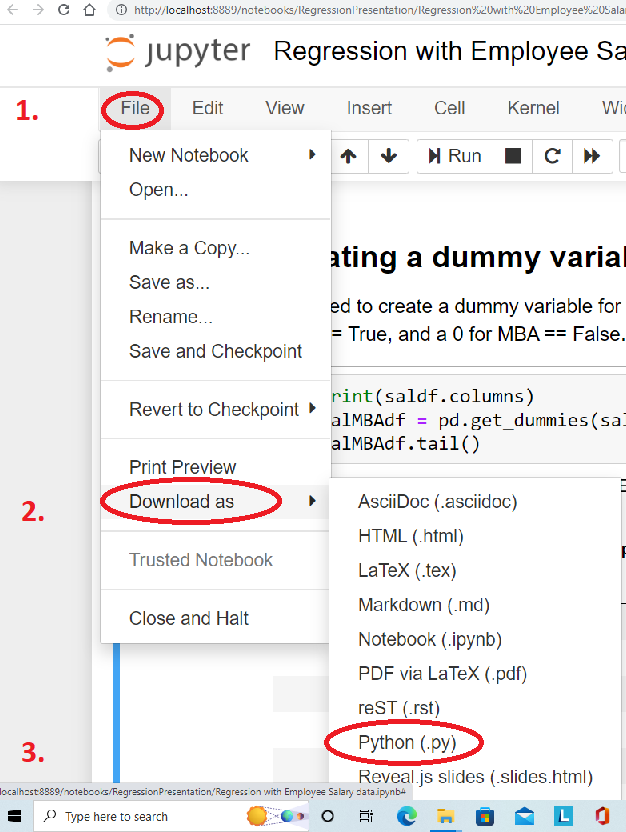
\includegraphics[width=2.5in]{DownloadAsPython.png}
            %\caption{Adding \ty{\_ViewImports.cshtml}}
            %\label{fig:asp07a}
        \end{center}
    \end{figure} 
\end{frame}

\begin{frame}
    \LARGE Gotchas

    \normalsize
    You need to \textbf{print()} everything you want to go to output.

    You cannot include your written analysis in the script (unless you print it).

    You will need to run your script in the approprate environment, i.e., Anaconda.
    
\end{frame}

\section{User Input, IPyWidgets}



\begin{frame}
    \LARGE Getting user input in your notebook

    \normalsize
    Use the Jupyter Widgets library, ipywidgets.

    \url{https://ipywidgets.readthedocs.io/en/stable/ }

    \url{https://ipywidgets.readthedocs.io/en/stable/examples/Widget\%20List.html\# }

    \url{https://ipywidgets.readthedocs.io/en/7.x/examples/Widget\%20Low\%20Level.html }

    \url{https://www.tutorialspoint.com/jupyter/jupyter\_notebook\_ipywidgets.htm }
    
\end{frame}

\begin{frame}
    \LARGE Gotchas

    \normalsize
    This library isn't exactly mature.

    You will need to do a lot of end user handholding.

    This breaks the automation.

    
\end{frame}


\section{Questions}

\begin{frame}
    \LARGE Conclusions and Questions

    \normalsize
    Any questions?
\end{frame}


%\begin{frame}
%    \LARGE Introduction\\
%
%    \normalsize
%    \begin{enumerate}
%\item{Our chosen topic is important.}
%\item{Our topic is relevant and related to the human aspects of cybersecurity.}
%\item{We have significant need for new solutions for the problems related to out topic.}
%\item{We have a significant opportunity to learn new facts and aspects of the topic.}
%    \end{enumerate}
%
%\end{frame}
%
%
%\begin{frame}
%    \LARGE Analysis Framework\\
%
%    \normalsize
%    \begin{itemize}
%        \item Laws and Regulations
%        \item Societal Norms
%        \item Markets and Economic Forces
%        \item Technical Means
%    \end{itemize}
%
%\end{frame}
%
%\begin{frame}
%    \LARGE Schedule\\
%
%    \normalsize
%    \begin{center}
%    \begin{tabular}{ | l | l |}
%        \hline
%        October 16 & Complete review of research sources \\
%        \hline
%        October 23 & First draft of research paper \\
%        \hline
%        October 30 & Second draft of research paper \\
%        \hline
%        November 6 & Third draft of research paper \\
%        \hline
%        November 13 & Final draft of research paper \\
%        \hline
%        November 20 & Final draft of presentation \\
%        \hline
%        November 27 & Final review and rehearsal of presentation \\
%        \hline
%        December 4 & Class presentation of research \\
%        \hline
%    \end{tabular}
%    \end{center}
%    
%\end{frame}
%
%
%\begin{frame}
%    \LARGE Questions and Feedback\\
%
%\end{frame}


\end{document}

